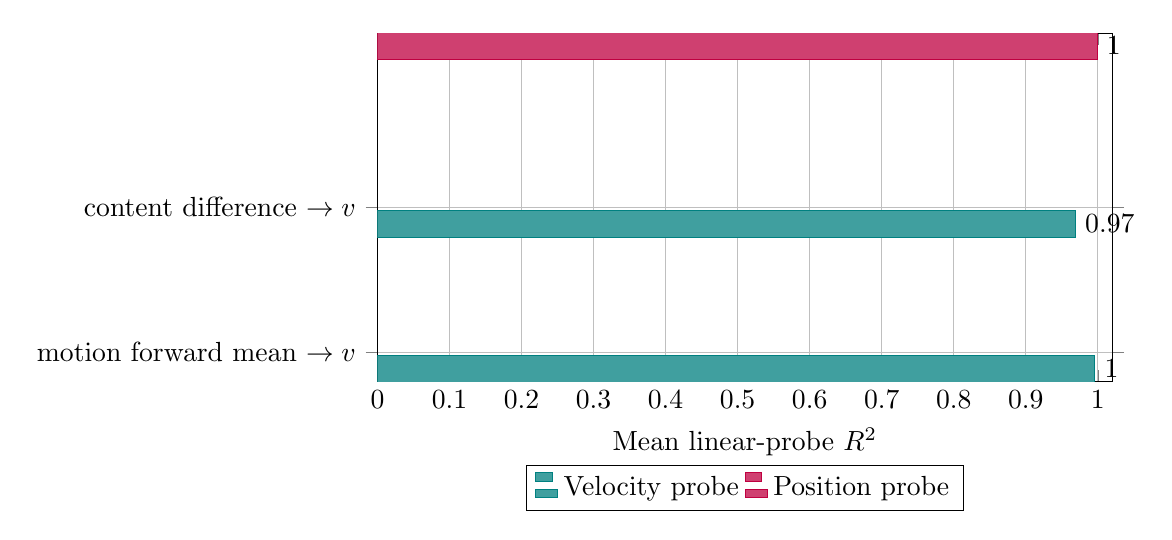
\begin{tikzpicture}
\begin{axis}[xbar,width=.9\textwidth,height=6cm,xmin=0,xmax=1.02,xlabel={Mean linear-probe $R^2$},symbolic y coords={motion forward mean $\to v$,content difference $\to v$,content last $\to p$},ytick=data,nodes near coords,grid=major,legend style={at={(0.5,-0.24)},anchor=north,legend columns=2}]
\addplot[fill=teal!75,draw=teal] coordinates {(0.996,motion forward mean $\to v$) (0.969,content difference $\to v$)};
\addplot[fill=purple!75,draw=purple] coordinates {(0.999,content last $\to p$)};
\legend{Velocity probe,Position probe}
\end{axis}
\end{tikzpicture}
